133. \begin{figure}[ht!]
\center{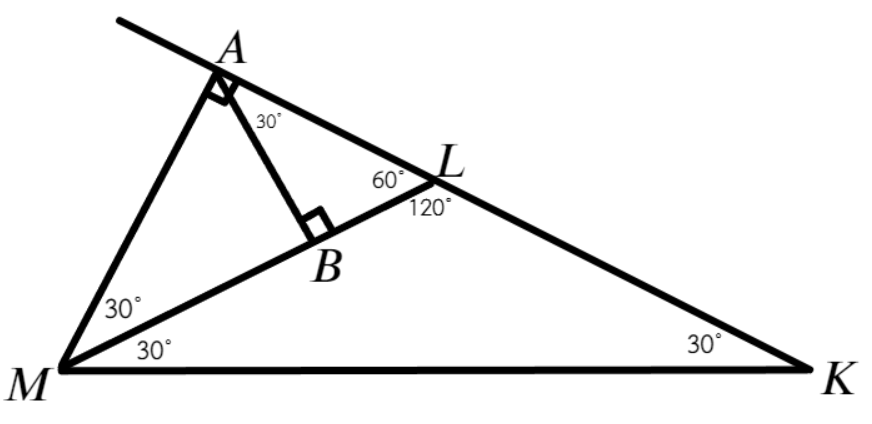
\includegraphics[scale=0.35]{g7-133.png}}
\end{figure}\\
Найдём $\angle BLA=180^\circ-120^\circ=60^\circ,\ \angle AMB=\angle BAL=90^\circ-60^\circ=30^\circ.$ Так как треугольник $KLM$ равнобедренный, $ML=KL=6$см. По теореме о катете, лежащем напротив угла в $30^\circ,$ получим $LA=\cfrac{1}{2}LM=\cfrac{1}{2}\cdot6=3,\ BL=\cfrac{1}{2}LA=\cfrac{1}{2}\cdot3=1,5$см, поэтому $BM=6-1,5=4,5$см.\\
